\documentclass[aspectratio=169, table, 12pt]{beamer}

\usepackage{colortbl}
\usepackage{xcolor}
\usepackage{listings}
\usepackage{tabularx}
\usepackage{tikz}
\usetikzlibrary{arrows.meta, positioning, calc, fit, shapes.geometric}

\makeatletter
\def\input@path{{../theme/}}
\makeatother
\graphicspath{{../theme/}{../../figures/}}
\usetheme{Pradita}

\definecolor{praditagreen}{RGB}{37, 113, 71}

% Tema membuat garis tabel berwarna putih. Dikembalikan agar tabel terbaca.
\arrayrulecolor{black}
\setlength{\arrayrulewidth}{0.5pt}

% Menempatkan gambar di tengah kolom, mendatar sekaligus tegak. Lebarnya
% dipenuhi selebar kolom. Bila hasilnya melebihi tinggi yang disediakan,
% tingginya yang menjadi pembatas, sehingga gambar tidak menembus bingkai.
\newsavebox{\kotakkolom}
\newcommand{\gambarkolom}[2][0.72\textheight]{%
  \sbox{\kotakkolom}{\resizebox{\linewidth}{!}{#2}}%
  \begin{minipage}[c][#1][c]{\linewidth}%
    \centering
    \ifdim\dimexpr\ht\kotakkolom+\dp\kotakkolom\relax>#1\relax
      \resizebox{!}{#1}{#2}%
    \else
      \usebox{\kotakkolom}%
    \fi
  \end{minipage}%
}

\lstdefinestyle{PythonStyle}{
  language=Python,
  basicstyle=\ttfamily\scriptsize,
  keywordstyle=\color{blue}\bfseries,
  commentstyle=\color{gray}\itshape,
  stringstyle=\color{red},
  breaklines=true,
  frame=lines,
  backgroundcolor=\color{lightgray!10},
  tabsize=2,
  showstringspaces=false
}

\lstdefinelanguage{bash}{
  keywords={},
  basicstyle=\ttfamily\scriptsize,
  ndkeywords={cd, python, bash, source},
  ndkeywordstyle=\color{purple}\bfseries,
  sensitive=true,
  commentstyle=\color{gray},
  breaklines=true,
  frame=lines,
  backgroundcolor=\color{lightgray!10},
  tabsize=2,
  comment=[l]{\#},
  showstringspaces=false
}

\title{\Huge{Microkernel dan Plugin}}
\subtitle{IF231303 Arsitektur Perangkat Lunak}
\author{Alfa Yohannis}

\begin{document}

\frame{\titlepage}

\begin{frame}{{\Large Tujuan Pembelajaran}}
  \vspace{10pt}
  \begin{enumerate}
    \item Menjelaskan pembagian antara inti dan \textit{plugin} beserta kontrak
          yang menghubungkan keduanya.
    \item Membedakan aktivasi awal dari aktivasi lambat, lalu menentukan kapan
          masing-masing layak dipilih.
    \item Mengukur penyebutan \textit{plugin} di dalam inti, akibat satu
          \textit{plugin} rusak, dan selisih waktu siap kedua cara aktivasi.
  \end{enumerate}

  \vspace{10pt}
  {\small Bab ini menyinggung sistem operasi sekilas, lalu menitikberatkan
  arsitektur \textit{plugin} pada perkakas sehari-hari.}
\end{frame}

\begin{frame}{{\Large Pendahuluan}}
  \vspace{8pt}
  \begin{itemize}\small
    \item Microkernel memisahkan sistem menjadi inti kecil beserta bagian
          tambahan yang dapat dipasang dan dicabut.
    \item Istilahnya lahir di sistem operasi, tetapi bentuk yang paling sering
          ditemui adalah turunannya, yaitu arsitektur \textit{plugin}.
    \item Eclipse, Visual Studio Code, Chrome, dan Firefox memakainya. Inti
          keempatnya kecil, dan hampir seluruh kemampuan datang dari luar.
  \end{itemize}

  \vspace{8pt}
  {\small Pertanyaannya bukan bagaimana menulis kernel, melainkan bagaimana
  sebuah inti menerima kemampuan baru tanpa mengenal satu pun penyumbangnya.}
\end{frame}

\begin{frame}{{\Large Inti Kecil, \textit{Plugin} Banyak}}
  \vspace{10pt}
  \centering
  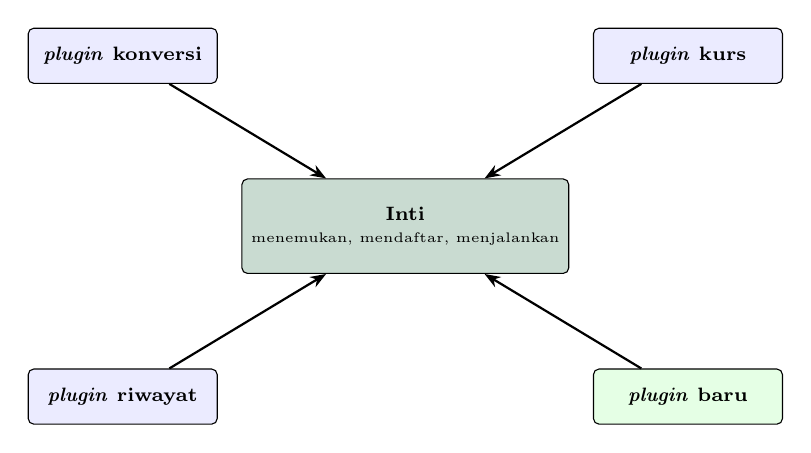
\begin{tikzpicture}[
    kotak/.style={draw, rounded corners=2pt, minimum width=2.4cm,
      minimum height=0.7cm, align=center, font=\scriptsize\bfseries},
    panah/.style={-{Stealth[length=2mm]}, thick}
  ]
    \node[kotak, fill=praditagreen!25, minimum width=3.6cm,
      minimum height=1.2cm] (inti) {Inti\\
      {\tiny\mdseries menemukan, mendaftar, menjalankan}};
    \node[kotak, fill=blue!8, above left=1.2cm and 0.3cm of inti] (p1)
      {\textit{plugin} konversi};
    \node[kotak, fill=blue!8, above right=1.2cm and 0.3cm of inti] (p2)
      {\textit{plugin} kurs};
    \node[kotak, fill=blue!8, below left=1.2cm and 0.3cm of inti] (p3)
      {\textit{plugin} riwayat};
    \node[kotak, fill=green!10, below right=1.2cm and 0.3cm of inti] (p4)
      {\textit{plugin} baru};
    \draw[panah] (p1) -- (inti);
    \draw[panah] (p2) -- (inti);
    \draw[panah] (p3) -- (inti);
    \draw[panah] (p4) -- (inti);
  \end{tikzpicture}

  \vspace{8pt}
  {\small Seluruh panah menunjuk ke dalam. Menambah kotak baru karena itu tidak
  menyentuh isi inti.}
\end{frame}

\begin{frame}[fragile]{{\Large Kontrak yang Ditulis Inti}}
  \vspace{6pt}
  {\small Inti menulis kontraknya, \textit{plugin} yang mengisinya. Eclipse
  menyebut kontrak itu \textit{extension point}.}
  \vspace{4pt}
\begin{lstlisting}[style=PythonStyle]
KUNCI_MANIFES = ("nama", "perintah", "keterangan", "modul", "kelas")

class Plugin(Protocol):
  def __init__(self, inti: object) -> None: ...
  def jalankan(self, argumen: list[str]) -> str: ...
\end{lstlisting}
  \vspace{4pt}
  \begin{itemize}\small
    \item Kontraknya sengaja kecil, sebab kontrak gemuk menyulitkan penulis
          \textit{plugin}.
    \item Manifes disimpan sebagai berkas JSON terpisah, sehingga dapat dibaca
          tanpa mengimpor kodenya.
  \end{itemize}
\end{frame}

\begin{frame}{{\Large Diagram Kelas Inti dan \textit{Plugin}}}
  \vspace{2pt}
  \begin{columns}[c]
    \begin{column}{0.52\textwidth}
      \gambarkolom{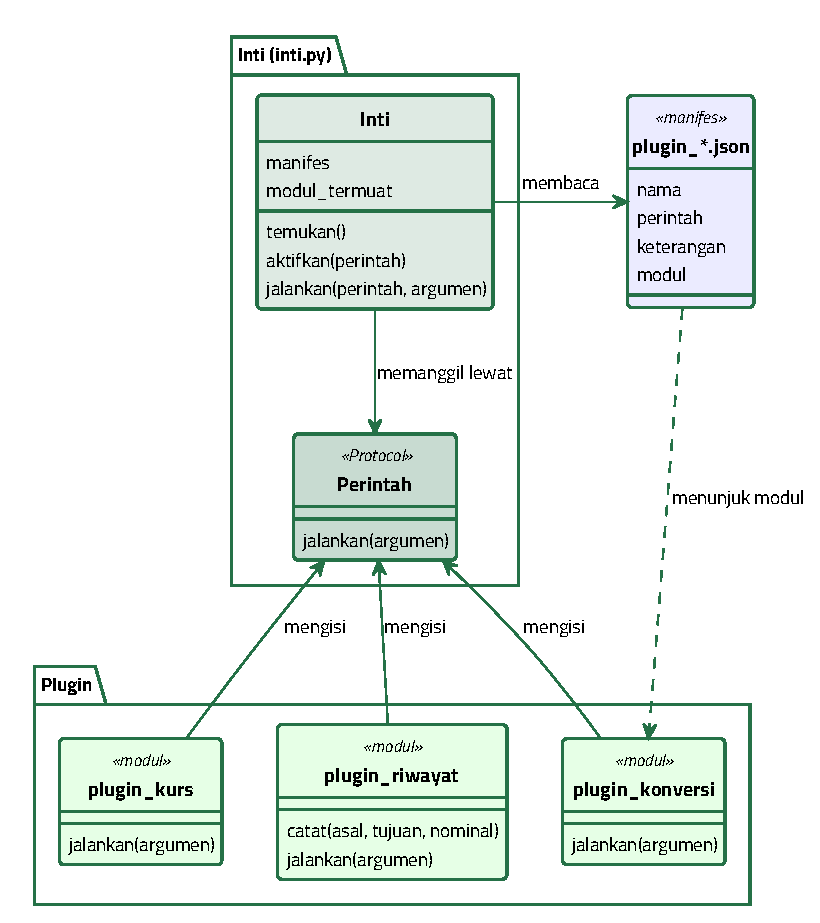
\includegraphics{kelas-microkernel.pdf}}
    \end{column}
    \begin{column}{0.46\textwidth}
      \begin{itemize}\small
        \item Panah dari inti hanya menuju kontrak dan manifes.
        \item Ketiga \textit{plugin} mengisi kontrak yang sama, dan tidak saling
              mengenal.
        \item Manifeslah yang menunjuk nama modulnya, bukan kode inti.
        \item Menambah \textit{plugin} berarti menambah dua berkas, yaitu modul
              dan manifesnya.
      \end{itemize}
    \end{column}
  \end{columns}
\end{frame}

\begin{frame}{{\Large Manifes pada Empat Produk}}
  \vspace{8pt}
  \centering
  \small
  \begin{tabularx}{0.95\textwidth}{|l|l|X|}
    \hline
    \textbf{Produk} & \textbf{Manifes} & \textbf{Catatan} \\
    \hline
    Eclipse & \texttt{plugin.xml} & Kontraknya \textit{extension point}, pengisinya \textit{extension} \\
    \hline
    Visual Studio Code & \texttt{package.json} & Dimuat saat \textit{activation event} terjadi \\
    \hline
    Chrome & \texttt{manifest.json} & \textit{Content script} di \textit{isolated world} terpisah \\
    \hline
    Firefox & \texttt{manifest.json} & Model WebExtensions yang sama, dengan perbedaan yang disengaja \\
    \hline
  \end{tabularx}

  \vspace{8pt}
  {\small Namanya berbeda, susunannya sama. Ketiganya menyimpan manifes di luar
  kode dan menunda pemuatan.}
\end{frame}

\begin{frame}{{\Large Padanan pada Contoh Java}}
  \vspace{8pt}
  \centering
  \small
  \begin{tabularx}{0.95\textwidth}{|X|X|}
    \hline
    \textbf{Contoh Java} & \textbf{Contoh Python} \\
    \hline
    \texttt{plugin.properties} berisi \texttt{mainclass} & \texttt{plugin\_*.json} berisi \texttt{modul} dan \texttt{kelas} \\
    \hline
    \texttt{URLClassLoader}, \texttt{Class.forName} & \texttt{importlib.import\_module}, \texttt{getattr} \\
    \hline
    Konstruktor refleksi menerima \texttt{Greeter} & Konstruktor kelas menerima \texttt{Inti} \\
    \hline
  \end{tabularx}

  \vspace{8pt}
  {\small Kode Java-nya tersimpan di \texttt{java-example/} sebagai pembanding
  lintas bahasa. Refleksinya Python adalah \texttt{importlib}.}
\end{frame}

\begin{frame}{{\Large Aktivasi Lambat: Urutan Panggilan}}
  \vspace{4pt}
  \begin{center}
    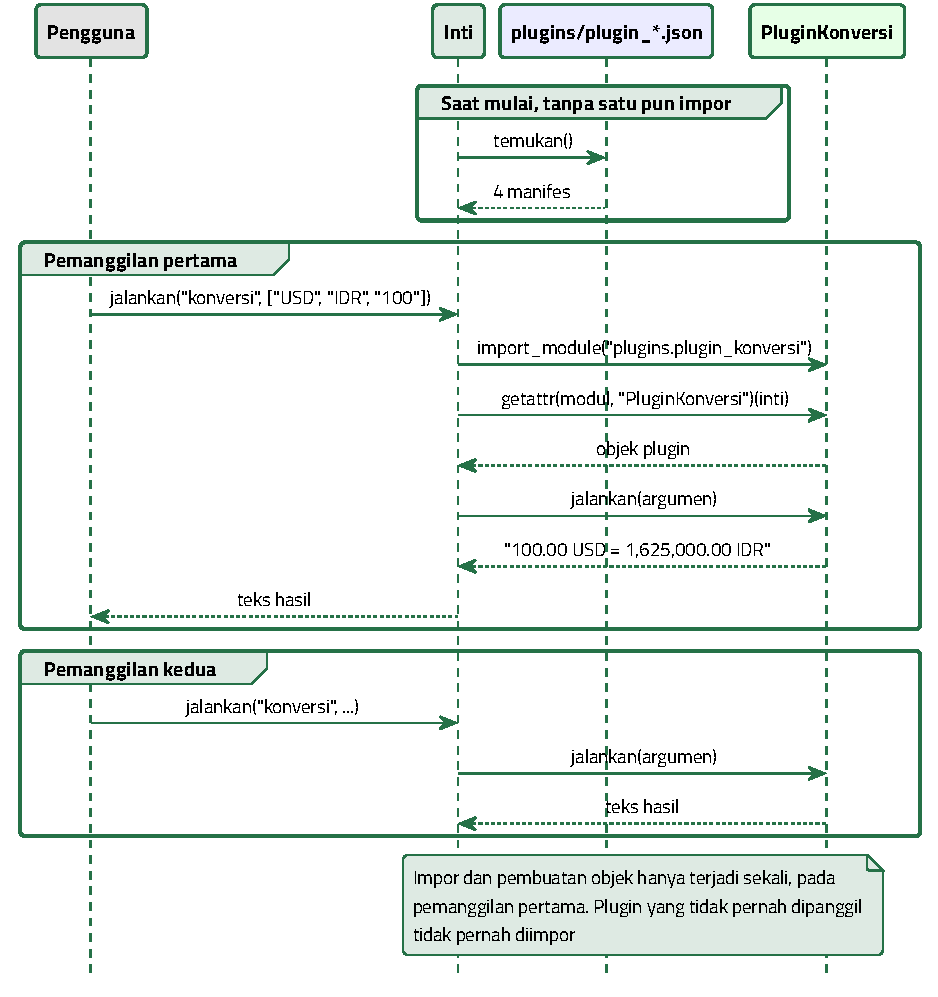
\includegraphics[width=\textwidth, height=0.64\textheight,
      keepaspectratio]{sekuens-aktivasi.pdf}
  \end{center}
  {\small Manifes dibaca saat mulai, modulnya diimpor pada pemanggilan pertama.
  \textit{Plugin} yang tidak pernah dipanggil tidak pernah diimpor.}
\end{frame}

\begin{frame}[fragile]{{\Large Aktivasi Dibungkus Penangkap Galat}}
  \vspace{6pt}
\begin{lstlisting}[style=PythonStyle]
def aktifkan(self, perintah: str) -> kontrak.Plugin:
  if perintah in self.plugin_aktif:
    return self.plugin_aktif[perintah]
  manifes = self.manifes[perintah]
  try:
    modul = importlib.import_module(manifes["modul"])
    kelas = getattr(modul, manifes["kelas"])
    plugin = kelas(self)          # inti diserahkan ke plugin
  except Exception as kesalahan:
    raise PluginGagal(f"{manifes['nama']} gagal dimuat: {kesalahan}")
  self.plugin_aktif[perintah] = plugin
  return plugin
\end{lstlisting}
  \vspace{4pt}
  {\small Hasil impor disimpan, sehingga pemanggilan kedua tidak membayar biaya
  yang sama. Galatnya dibungkus agar satu \textit{plugin} rusak tidak
  menjatuhkan inti.}
\end{frame}

\begin{frame}{{\Large Analogi: Kantin yang Menyewakan Kios}}
  \vspace{10pt}
  \begin{itemize}\small
    \item Pengelola menyediakan tempat, listrik, air, dan aturan jam buka.
    \item Siapa saja boleh membuka kios selama aturan itu dipenuhi.
    \item Pengelola tidak perlu tahu menu apa yang dijual, sebab yang diurusnya
          hanya daftar penyewa beserta papan namanya.
    \item Satu kios yang tutup tidak menutup kantinnya, sebab pembeli cukup
          berpindah ke kios sebelah.
  \end{itemize}

  \vspace{10pt}
  {\small Aturan jam buka itulah kontraknya, papan nama itulah manifesnya, dan
  daftar penyewa itulah registrinya.}
\end{frame}

\begin{frame}{{\Large Kasus: Lima \textit{Plugin}, Satu Berkas Hilang}}
  \vspace{8pt}
  \begin{enumerate}\small
    \item Sebuah tim memasang lima \textit{plugin}, seluruhnya diaktifkan saat
          aplikasi mulai.
    \item Satu \textit{plugin} membaca berkas pengaturan pada tingkat modul, di
          luar fungsi mana pun.
    \item Pada suatu pagi berkas itu terhapus, dan impornya gagal.
    \item Aplikasi tidak menampilkan galat satu \textit{plugin}, melainkan gagal
          mulai sama sekali.
  \end{enumerate}

  \vspace{8pt}
  {\small Empat \textit{plugin} sehat ikut mati, dan pengguna tidak dapat
  menonaktifkan yang rusak, sebab layarnya tidak pernah muncul.}
\end{frame}

\begin{frame}{{\Large Hasil Pengukuran}}
  \vspace{8pt}
  \centering
  \small
  \begin{tabularx}{0.9\textwidth}{|X|l|}
    \hline
    \textbf{Yang dilaporkan} & \textbf{Nilai} \\
    \hline
    Median aktivasi lambat & 0,4006 ms \\
    \hline
    Median aktivasi awal & 1,3406 ms \\
    \hline
    Selisih median antar jalur & 0,9399 ms \\
    \hline
    Aktivasi awal lebih lambat & 3,3 kali \\
    \hline
    \textit{Range} dibagi selisih & 0,3 kali \\
    \hline
    Putaran lambat lebih cepat & 100 dari 100 \\
    \hline
  \end{tabularx}

  \vspace{8pt}
  {\small Berbeda dengan Bab 2, \textit{range}-nya lebih kecil daripada
  selisihnya. Selisih seperti inilah yang layak dilaporkan.}
\end{frame}

\begin{frame}{{\Large Ringkasan}}
  \vspace{10pt}
  \begin{itemize}\small
    \item Inti menulis kontrak dan membaca manifes, sedangkan \textit{plugin}
          yang mengisi kontrak itu.
    \item Karena inti tidak menyebut satu nama penyumbang pun, menambah
          kemampuan berarti menambah berkas.
    \item Manifes yang terpisah membuka pilihan kapan sebuah \textit{plugin}
          diaktifkan.
    \item Satu \textit{plugin} yang gagal saat impor dapat menjatuhkan seluruh
          aplikasi bila pemanggilannya tidak dibungkus.
  \end{itemize}

  \vspace{10pt}
  {\small Pesan utamanya bukan inti harus kecil, melainkan inti harus buta
  terhadap penyumbangnya.}
\end{frame}

\begin{frame}[fragile]{{\Large Persiapan Latihan}}
  \vspace{5pt}
\begin{lstlisting}[language=bash]
bash sources/siapkan_venv.sh
source .venv/bin/activate
cd sources/chapter05
python inti.py daftar
# Plugin terpasang: 4
# Plugin yang sudah aktif: 0
\end{lstlisting}

  \vspace{8pt}
  {\small Satu inti, empat \textit{plugin}, tiga masalah berbeda. Manifes dibaca
  saat mulai, sedangkan modulnya belum satu pun diimpor.}
\end{frame}

\begin{frame}[fragile]{{\Large Latihan 1: Menghitung Penyebutan \textit{Plugin}}}
  \vspace{3pt}
\begin{lstlisting}[language=bash]
python periksa_inti.py
# Plugin disebut inti    : 0 []
\end{lstlisting}

  \vspace{3pt}
  \begin{enumerate}\small
    \item Catat baris \texttt{Plugin disebut inti} beserta ketiga angka di
          bawahnya.
    \item Salin \texttt{plugins/plugin\_riwayat.py} beserta manifesnya menjadi
          \texttt{plugin\_pajak.py}, lalu ubah nama, perintah, dan kelasnya.
    \item Jalankan ulang keduanya, lalu catat berapa baris inti yang berubah.
  \end{enumerate}

  \vspace{3pt}
  {\small Pertanyaan: baris inti tidak berubah sama sekali. Bagian inti mana
  yang membuat hal itu mungkin?}
\end{frame}

\begin{frame}[fragile]{{\Large Latihan 2: Menjatuhkan Aplikasi}}
  \vspace{3pt}
\begin{lstlisting}[language=bash]
python uji_isolasi.py
# Dengan pelindung  : 3 perintah jalan, 1 dilewati
# Tanpa pelindung   : 3 modul terimpor, lalu berhenti
\end{lstlisting}

  \vspace{3pt}
  \begin{enumerate}\small
    \item Tunjukkan baris pada \texttt{plugins/plugin\_rusak.py} yang
          menyebabkan kegagalannya.
    \item Jalankan \texttt{python inti.py rusak} lalu \texttt{python inti.py
          kurs}, dan catat apakah perintah kedua tetap dilayani.
    \item Hapus sementara pembungkus galat di \texttt{inti.py}, lalu catat
          akibatnya.
  \end{enumerate}

  \vspace{3pt}
  {\small Pertanyaan: mengapa kegagalan saat impor lebih berbahaya daripada
  kegagalan saat pemanggilan?}
\end{frame}

\begin{frame}[fragile]{{\Large Latihan 3: Mengukur Biaya Aktivasi Awal}}
  \vspace{3pt}
\begin{lstlisting}[language=bash]
python ukur_aktivasi.py
# Putaran lambat lebih cepat   : 100 dari 100
\end{lstlisting}

  \vspace{3pt}
  \begin{enumerate}\small
    \item Catat kedelapan angka pada laporan akhirnya.
    \item Tunjukkan baris yang membersihkan cache impor.
    \item Hapus sementara pembersihan itu, jalankan ulang, lalu catat perubahan
          angkanya.
  \end{enumerate}

  \vspace{3pt}
  {\small Pertanyaan: mengapa selisih pada bab ini layak disebut ada, sedangkan
  selisih pada Bab 2 tidak?}
\end{frame}

\end{document}
